\documentclass[11  pt]{exam} 
\usepackage[lmargin=1in,rmargin=1.75in,bmargin=1in,tmargin=1in]{geometry}  


% For hyperlinking everything
\usepackage{hyperref}
\hypersetup{
	colorlinks=true, %set true if you want colored links
	linktoc=all,     %set to all if you want both sections and subsections linked
	linkcolor=blue,  %choose some color if you want links to stand out
}


\usepackage[latin1]{inputenc}
\usepackage{amsmath}
\usepackage{mathrsfs}  
\usepackage{amsfonts}
\usepackage{amssymb}
\usepackage{graphicx}
\usepackage{subfig}
\usepackage{caption}
\usepackage{algorithm}
%\usepackage{algcompatible}
%\usepackage{algorithmicx}
\usepackage{algpseudocode}

\usepackage{titlesec}
\titleformat{\section}{\fontfamily{lmss}\fontsize{14}{15}\bfseries}{\thesection}{1em}{}
\titleformat{\subsection}{\fontfamily{lmss}\fontsize{12}{15}\bfseries}{\thesubsection}{1em}{}




\usepackage{amsthm}

\newtheoremstyle{noit}
{10pt}% <Space above>
{10pt}% <Space below>
{}% <Body font>
{}% <Indent amount>
{\bfseries}% <Theorem head font>
{.}% <Punctuation after theorem head>
{.5em}% <Space after theorem headi>
{}% <Theorem head spec (can be left empty, meaning `normal')>

\newtheoremstyle{example}
{10pt}% <Space above>
{10pt}% <Space below>
{}% <Body font>
{20pt}% <Indent amount>
{\bfseries}% <Theorem head font>
{.}% <Punctuation after theorem head>
{.5em}% <Space after theorem headi>
{}% <Theorem head spec (can be left empty, meaning `normal')>


\newtheoremstyle{indented}{20pt}{20pt}{\addtolength{\leftskip}{2.5em}}{}{\bfseries}{.}{.5em}{}


\newtheorem{theorem}{Theorem}
\numberwithin{theorem}{section}
\newtheorem{lemma}[theorem]{Lemma}
\newtheorem{corollary}[theorem]{Corollary}
\newtheorem{observation}{Observation}
%\numberwithin{observation}{section}
%\numberwithin{definition}{section}
\newtheorem{conjecture}{Conjecture}
\newtheorem{Qu}{Question}
\newcommand{\QU}{\begin{Qu}\normalfont}

\theoremstyle{noit}
\newtheorem{fact}{Fact}
\newtheorem{definition}{Definition}

\theoremstyle{indented}
\newtheorem{example}{Example}

\theoremstyle{indented}
\newtheorem{problem}{Problem}


%\newenvironment{proof}{\noindent{\bf Proof:} \hspace*{1em}}{
%    \hspace*{\fill} $\Box$ }
%\newenvironment{proof_of}[1]{\noindent {\bf Proof of #1:}
%    \hspace*{1em} }{\hspace*{\fill} $\Box$ }
%\newenvironment{proof_claim}{\begin{quotation} \noindent}{
%    \hspace*{\fill} $\diamond$ \end{quotation}}
\newcommand{\vs}[1]{\vspace{#1}}

\newcommand{\lecture}[2]{
 \noindent
\begin{center}
	\framebox{
		\vbox{
			\hbox to 5.78in { {\bf CSCE 411: Design and Analysis of Algorithms} \hfill  }
			\vspace{2mm}
			\hbox to 5.78in { {\Large \hfill Lecture #1\hfill} }
			\vspace{2mm}
			\hbox to 5.78in { {\it Date: #2 \hfill Lecturer: Nate Veldt} }
		}
	}
\end{center}
\vspace*{4mm}
}


\newcommand{\hw}[2]{
	\noindent
	\begin{center}
		\framebox{
			\vbox{
				\hbox to 5.78in { {\bf CSCE 411: Design and Analysis of Algorithms} \hfill  }
				\vspace{2mm}
				\hbox to 5.78in { {\Large \hfill Homework #1\hfill} }
				\vspace{2mm}
				\hbox to 5.78in { {\it Due date: #2 \hfil} }
			}
		}
	\end{center}
	\vspace*{4mm}
}



\newcommand{\under}[1]{\underline{\hspace{#1}}}
\setlength{\parindent}{0em}

%\usepackage[tagged]{accessibility}

% Graph terms
\newcommand{\vol}{\textbf{vol}}
\newcommand{\cut}{\textbf{cut}}


% Matrices
\newcommand{\mA}{\textbf{A}}
\newcommand{\mB}{\textbf{B}}

% vectors
\newcommand{\ve}{\textbf{e}}
\newcommand{\vx}{\textbf{x}}


% Other
\newcommand{\calN}{\mathcal{N}}

\usepackage{mathtools}
\DeclarePairedDelimiter\ceil{\lceil}{\rceil}
\DeclarePairedDelimiter\floor{\lfloor}{\rfloor}


\newcommand*{\aitem}{ \item[{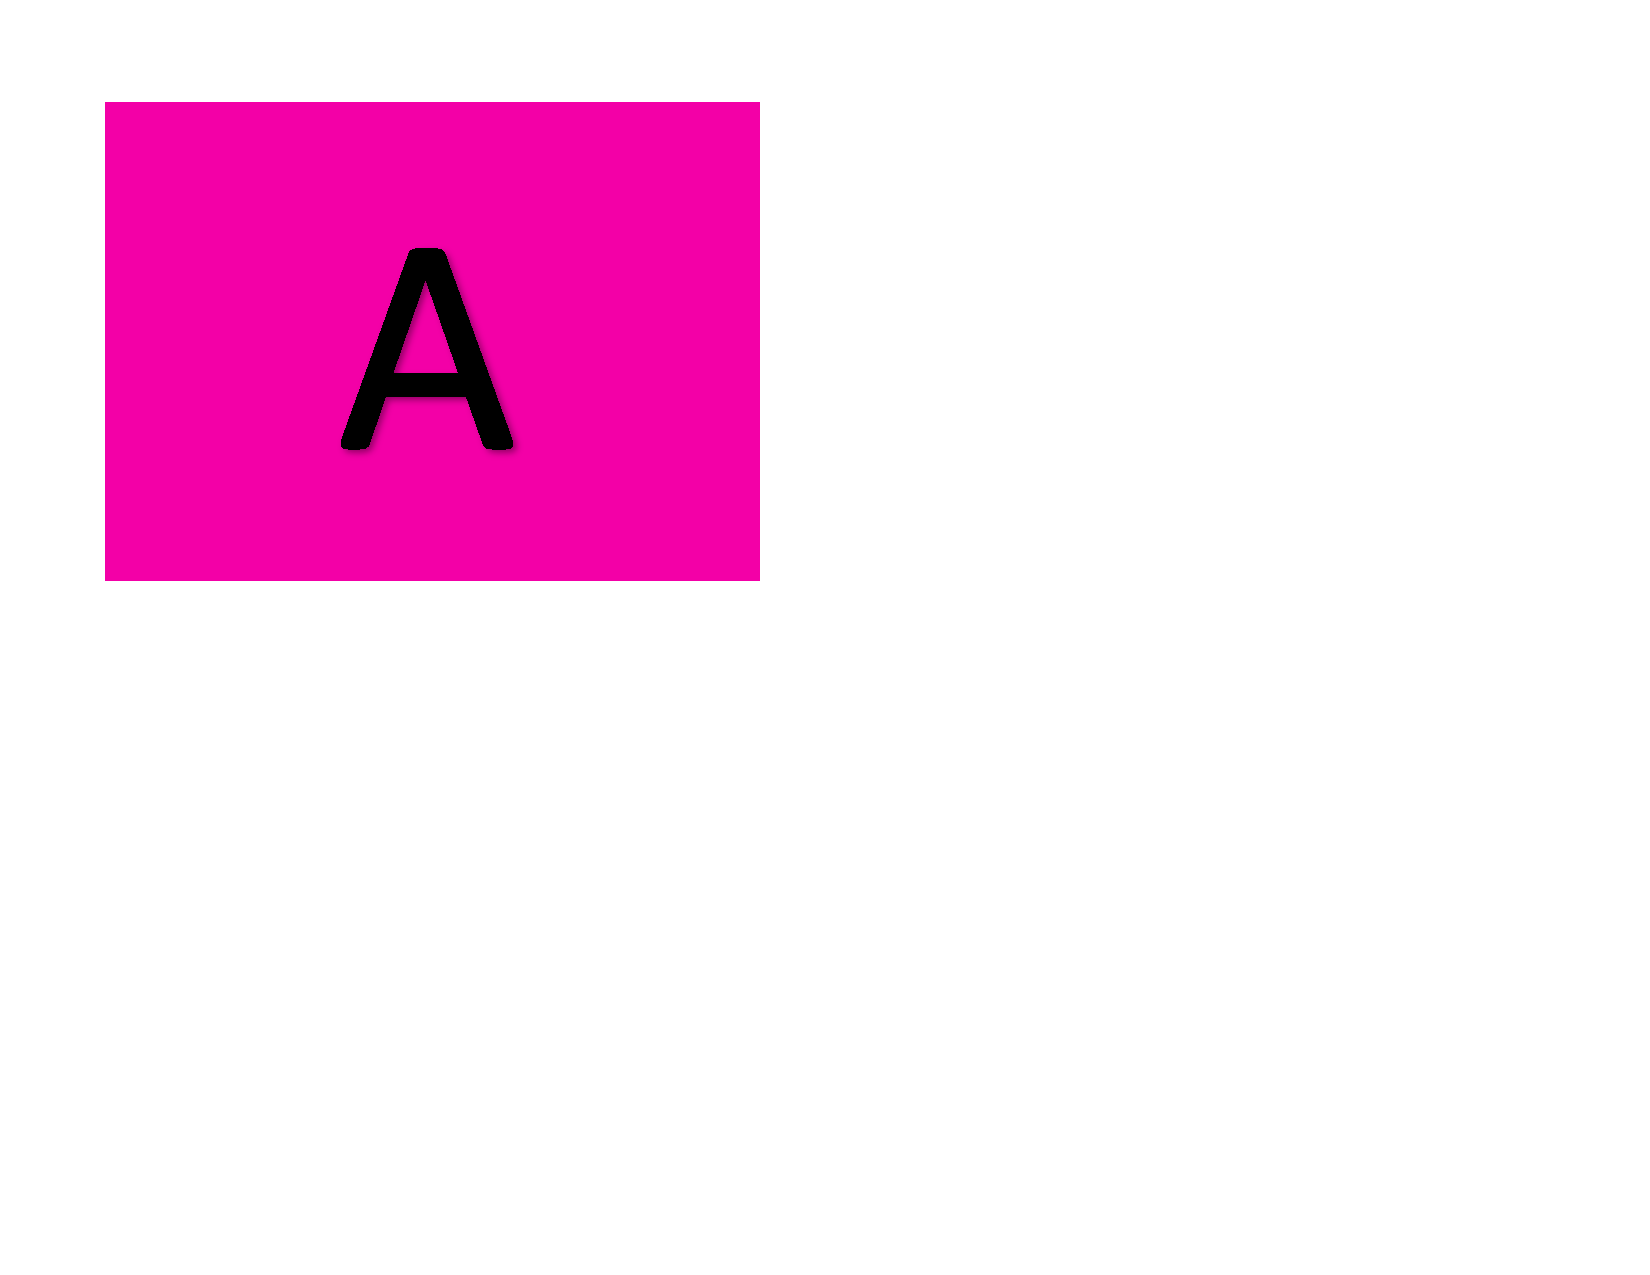
\includegraphics[width=0.8cm,height=0.5cm]{../../Lectures/figures/A}} ]  }
\newcommand*{\bitem}{ \item[{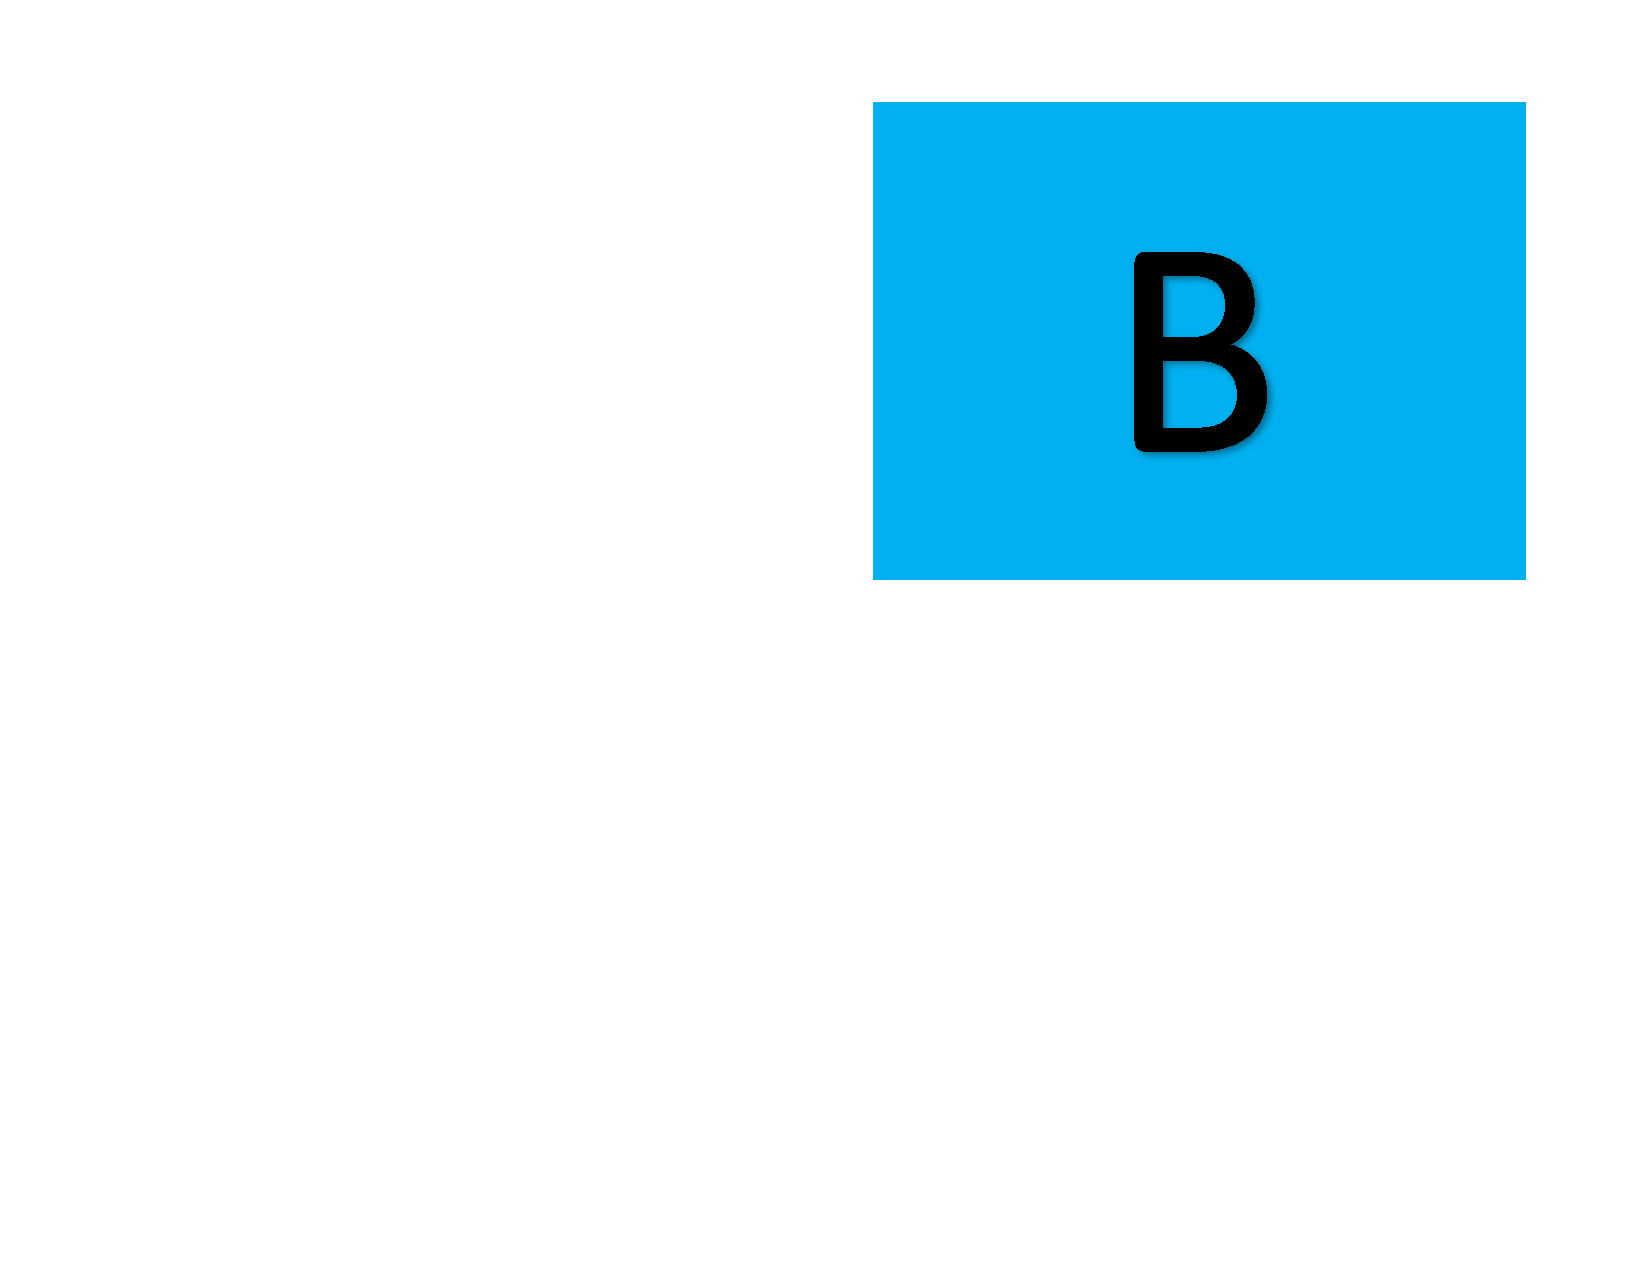
\includegraphics[width=0.8cm,height=0.5cm]{../../Lectures/figures/B}} ]  }
\newcommand*{\citem}{ \item[{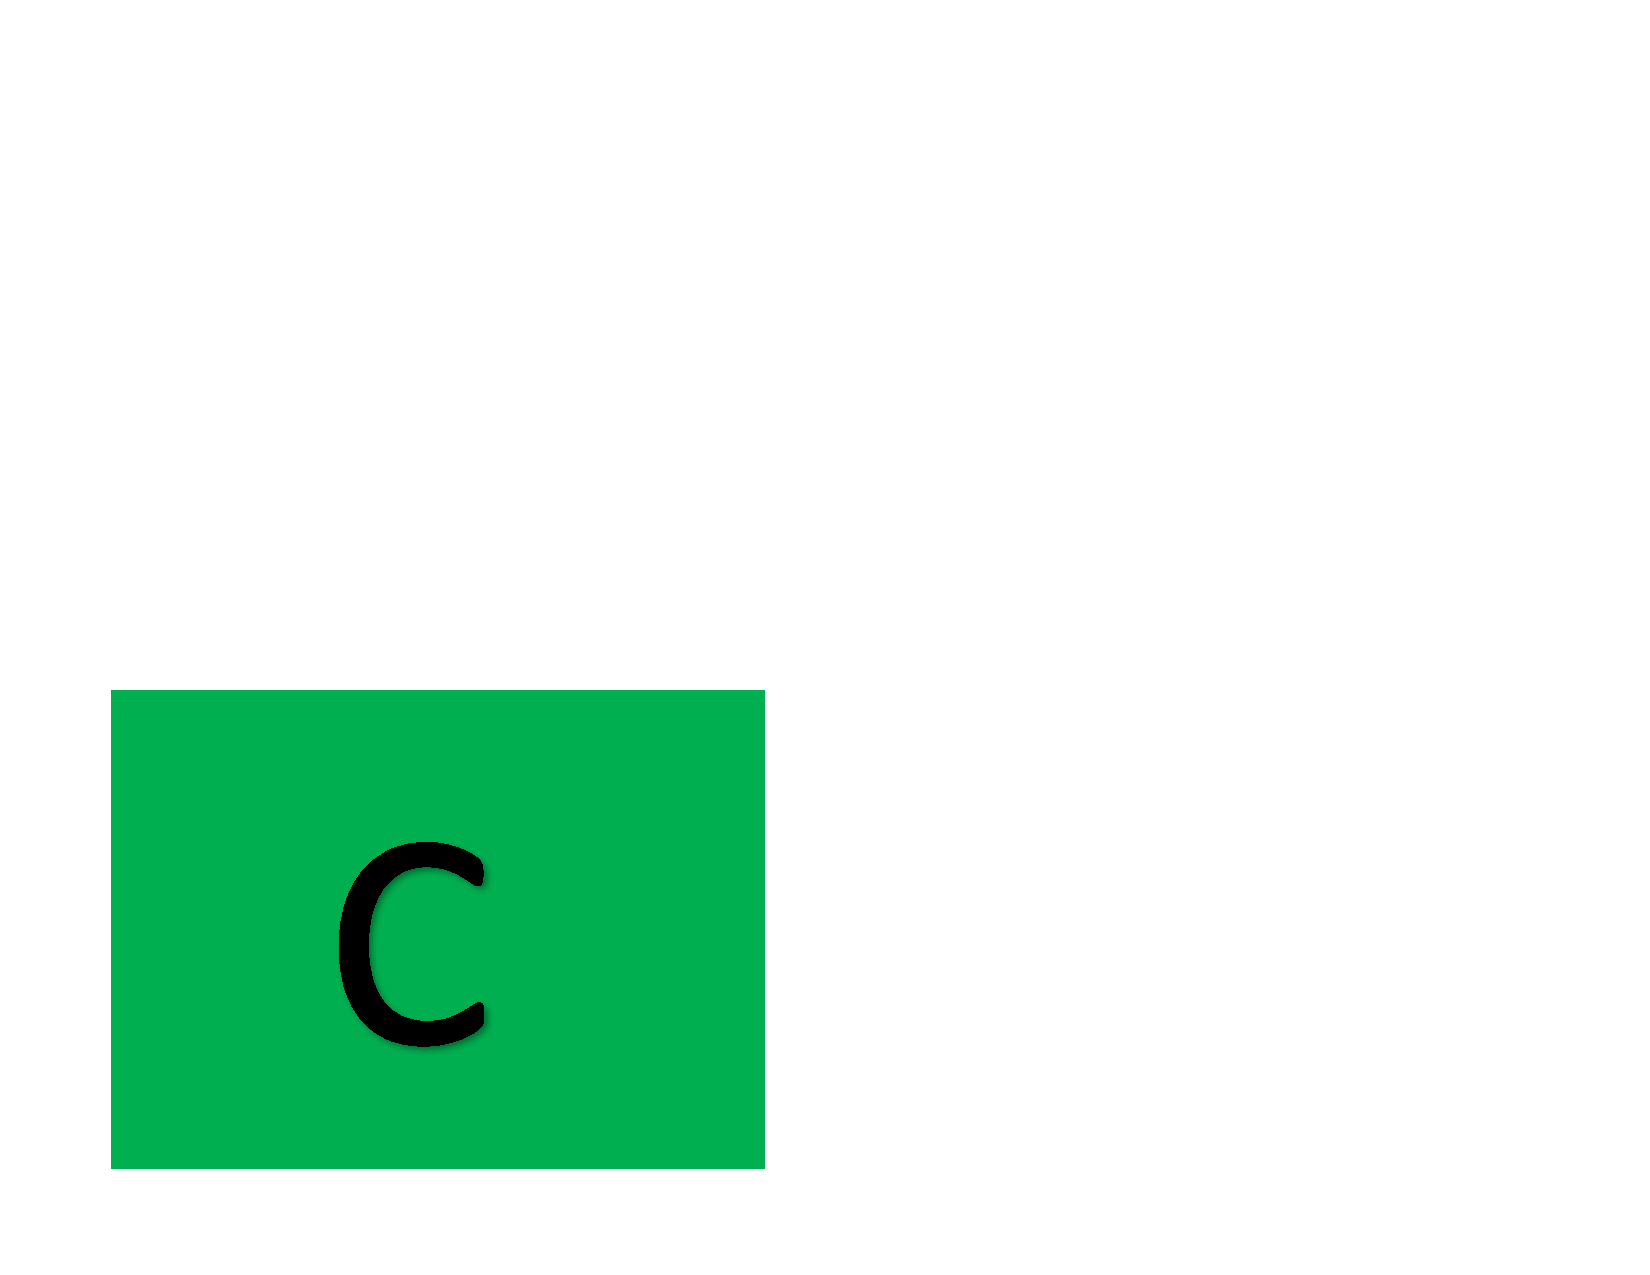
\includegraphics[width=0.8cm,height=0.5cm]{../../Lectures/figures/C}} ]  }
\newcommand*{\ditem}{ \item[{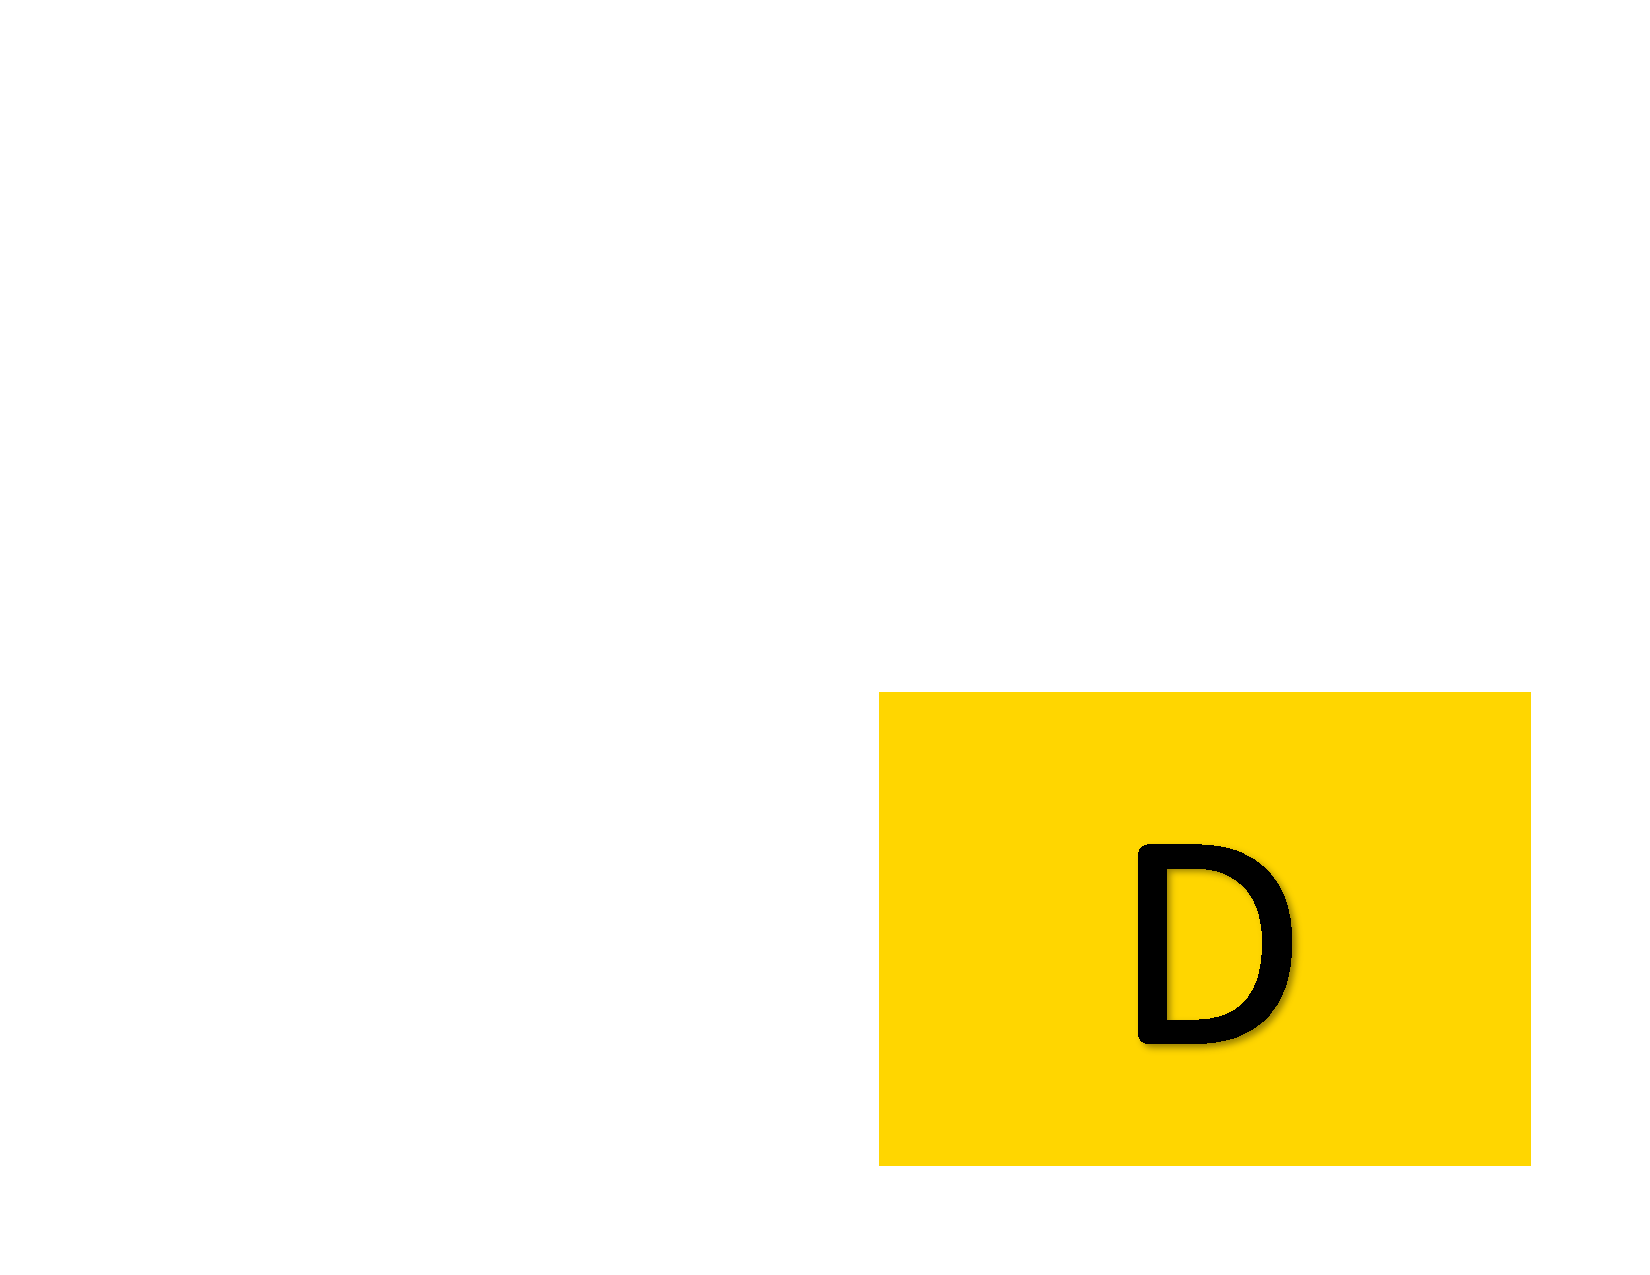
\includegraphics[width=0.8cm,height=0.5cm]{../../Lectures/figures/D}} ]  }
\newcommand*{\eitem}{ \item[{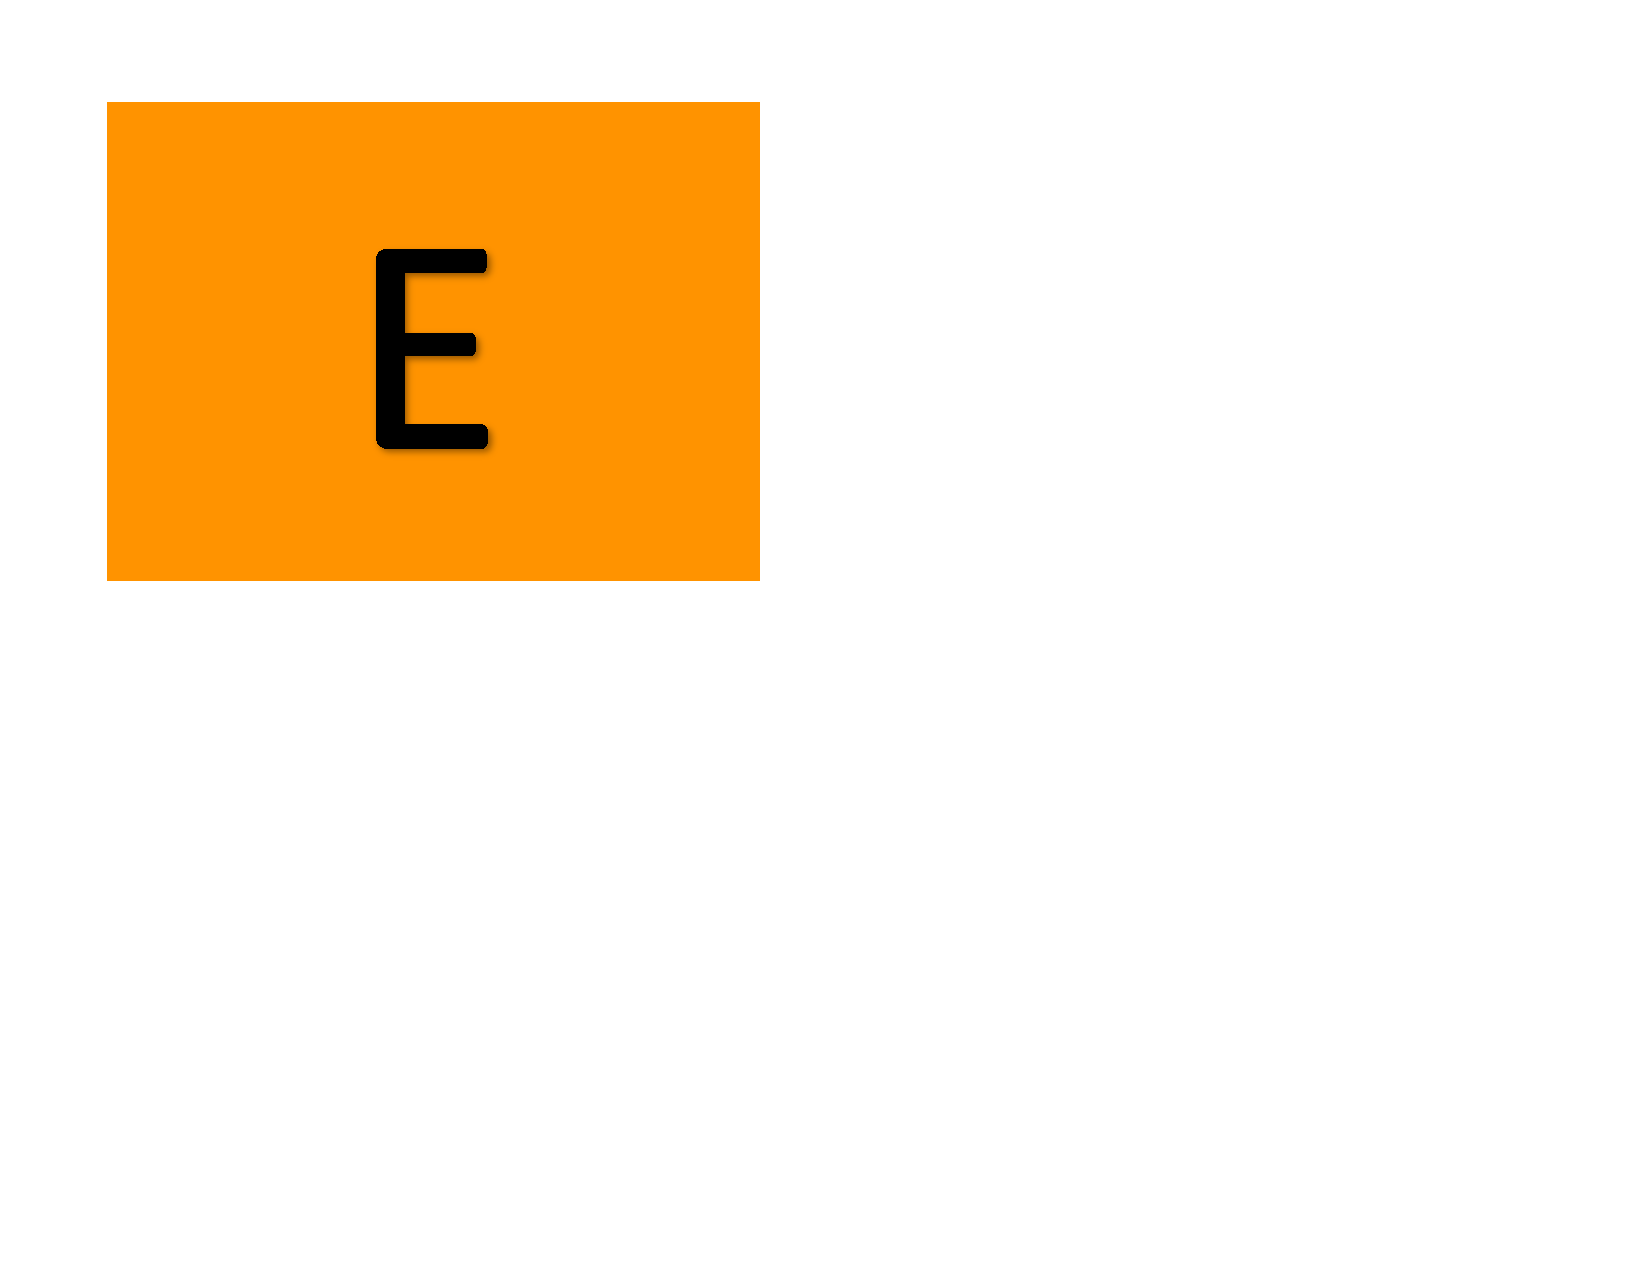
\includegraphics[width=0.8cm,height=0.5cm]{../../Lectures/figures/E}} ]  }
\newcommand*{\fitem}{ \item[{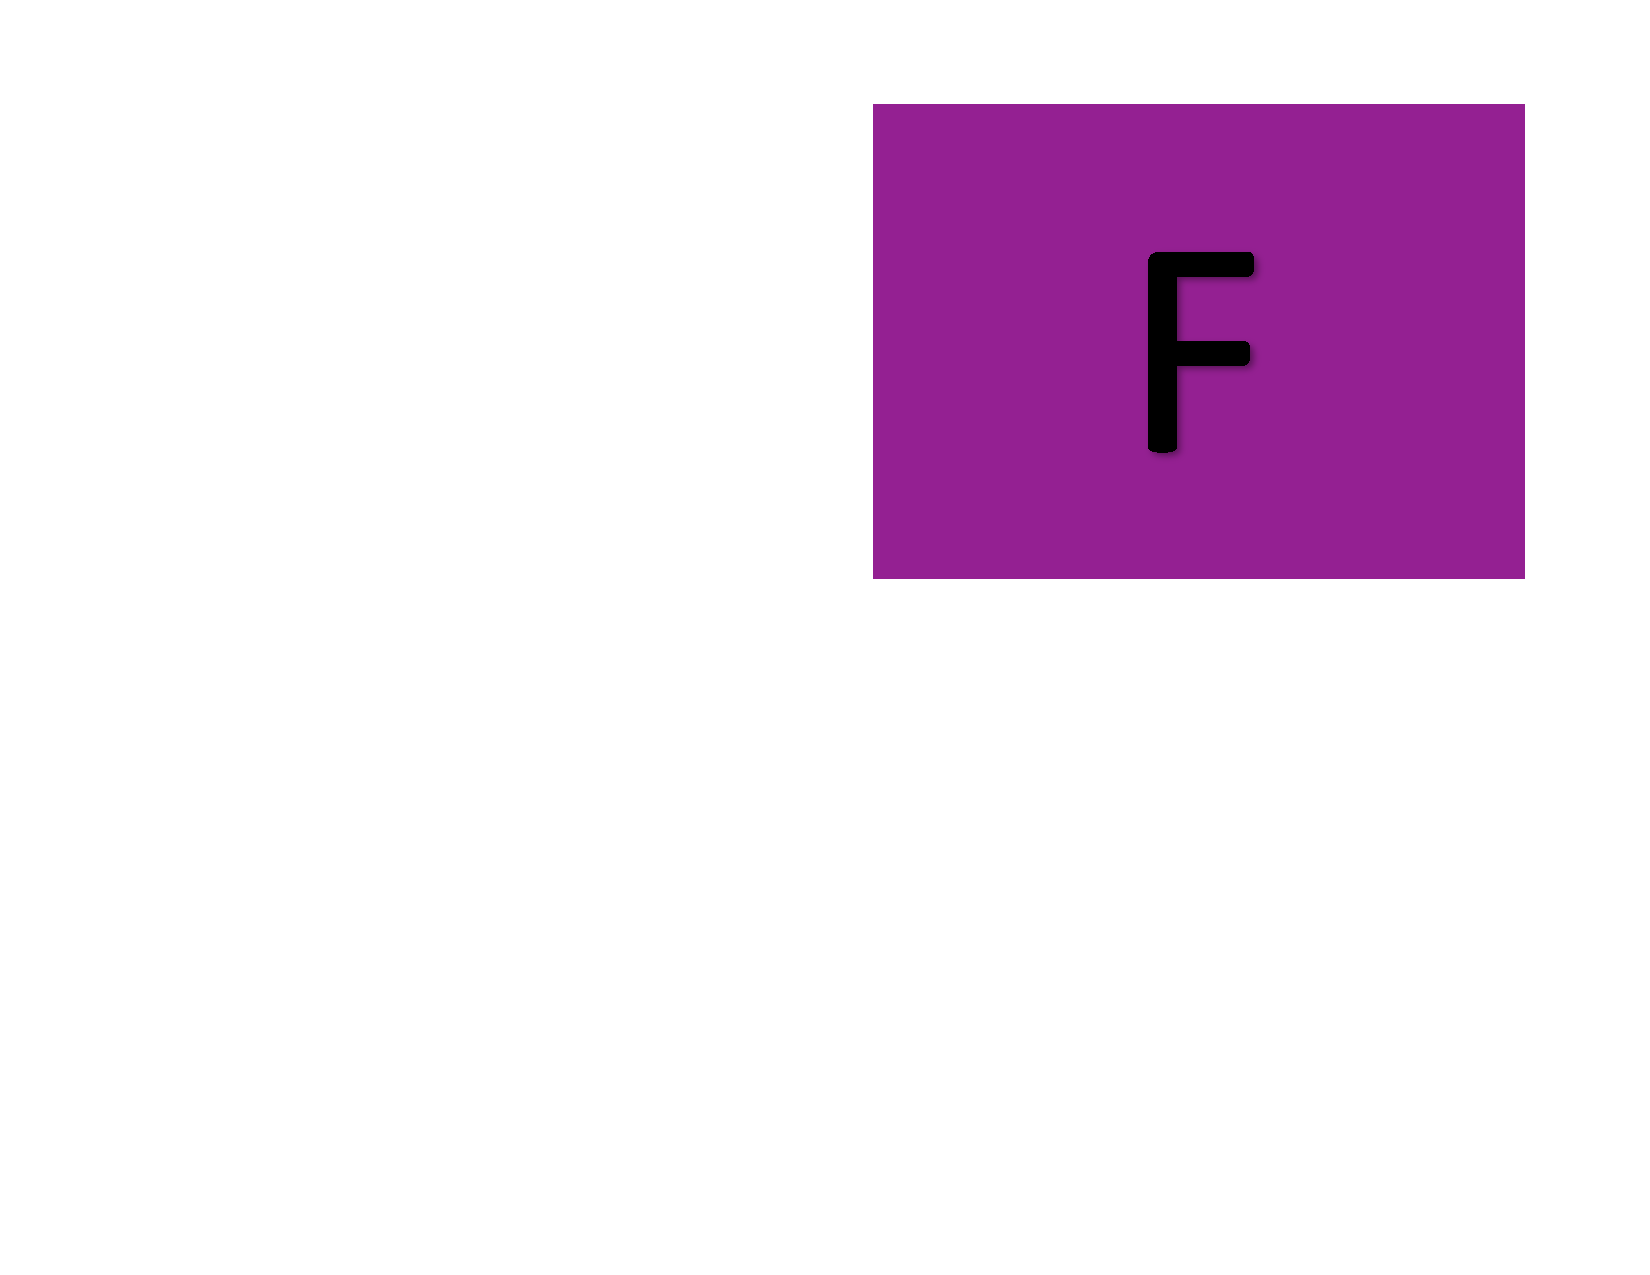
\includegraphics[width=0.8cm,height=0.5cm]{../../Lectures/figures/F}} ]  }


\newcommand{\hide}[1]{\underline{\phantom{#1 #1}}}

\usepackage{setspace}

\onehalfspacing

\begin{document}
	
	
	\lecture{19, Exam 2 Review}{April 1, 2025}
	
	%	\paragraph{Course Logistics}	
	%	\begin{itemize}
	%		\item First test is this Friday
	%	\end{itemize}
	
	\section{Test format and instructions}
	
	\begin{itemize}
		\item Some multiple choice questions, some long answer questions
		\item You do not need to prove something unless you are explicitly asked to prove something
		\item You may be asked to explicitly prove something 
		\item Scratch paper will be provided
		\item No calculators or electronic devices. You will not need them. If you have to do any computations, they will be basic enough to do by hand. 
		\item You will put your name on the front page, and put your initials at the top of every other page.
	\end{itemize}
	
%	{\Large  \centering This is all the same as Test 1!}
	
	A few other notes:
	\begin{itemize}
		\item If something was on a homework or in a lecture, it could be on the test.
		\item Some questions may involve a combination of a couple different things we've seen in different lectures.
		\item If we covered a proof of a result, you can reference it as fact without re-proving it, unless the question specifically is asking you to provide proof details.
	\end{itemize}
	
	\newpage 
	
	\section{Topics Covered on the Test}
	
	%	These notes go over the main topics we have studied, list questions for you to fill in that you should know about on the test, and give some examples of things you might be required to do on the test.
	%	
	\subsection{Summary of the summary}
	\begin{itemize}
		\item Graph basics (adjacency matrix, adjacency list, directed/undirected, weighted/unweighted, cyclic/acyclic)
		\item (BFS) Breadth-first search
		\item (DFS) Depth-first search (applications: strongly connected components, topological sort)
		\item (MST) Minimum spanning tree (Kruskal's and Prim's algorithms)
		\item (SSSP) Single source shortest paths (Bellman-Ford, Dijkstra's)
		\item Maximum $s$-$t$ flow and minimum $s$-$t$ cut
	\end{itemize}

For all of these graph algorithms, here's the short answer on what you should know:

\begin{itemize}
	\item How is the problem defined? In particular, what type of graph does it apply to? Are there restrictions?
	\item What algorithms solve the problem, what is their basic mechanism, and their runtime?
	\item Don't just know how to eye-ball a solution for a small graph. You should know the mechanics of each algorithm well enough that you could apply it to a small graph, could write out pseudocode if need be, and provide a runtime analysis 
\end{itemize}
	
\subsection{Graph Basics}
	
	\begin{itemize}
		\item Representing a graph as a list or a matrix
		\item Undirected and directed, weighted and unweighted (which of these can be viewed as special cases of others?)
		\item Strongly connected and weakly connected components. What is their relation? How are they defined?
		\item What is a bipartite graph?
	\end{itemize}

	\subsection{Breadth first search specifics}

	\begin{itemize}	
		\item Running a BFS on a weighted graph just means ignore the edge weights. (You wouldn't say ``BFS doesn't apply if the graph is weighted.'')
		\item Remember what a breadth-first tree is and how to find it.
		\item Make sure you know the runtime
	\end{itemize}


	\subsection{Depth-first search}
		\begin{itemize}	
			\item Know the different edge types in a depth-first search and what they mean
			\item Know the two main applications we discussed in class and how to use DFS for them.
		\end{itemize}

	\subsection{Minimum Spanning Tree}
\begin{itemize}	
	\item You should know the basic mechanism behind both Prim's and Kruskal's algorithm
	\item You should know what a cut is, and what a ``safe'' edge is.
	%\item We did a mini runtime analysis for Prim's algorithm: you should know what the runtime is and how that basic argument worked (there are many other algorithms with similar types of runtime analyses).
\end{itemize}

	\subsection{Single source shortest paths algorithm}

\begin{itemize}	
	\item Two algorithms we saw: Bellman-Ford, Dijkstra's %(and we talked about two ways to implement the min-priority queue).
	\item You should understand the basic mechanism behind each, and different pros/cons of their runtimes
\end{itemize}

	\subsection{Min-cut Max-Flow Problem and algorithms}

	\begin{itemize}	
		\item What is the definition of an $s$-$t$ flow function? What is an $s$-$t$ cut in a directed graph?
		\item What is the basic idea behind the algorithms we have seen? Hint: it isn't that you repeatedly try to send flow from $s$ to $t$ as long as you can find unsaturated paths in the original graph $G$. 
		%What is an augmenting path and a residual graph? 
%		\item What is the basic mechanism behind Ford-Fulkerson? What's it's runtime and why?
%		\item What is the difference between Ford-Fulkerson and Edmonds-Karp? What is the runtime difference? 
%		\item You would not be expected to reproduce a long proof such as the one we did for Edmond's Karp, but you might be expected to understand/explain one small subset.
%		\item You should know that what the maximum-flow minimum-cut theorem says and how to use it to verify that a flow or cut is optimal or not optimal.
	\end{itemize}

	\section{Practice Problems}
	
	\begin{questions}
		
		\question When does breadth-first search solve the same problem as Dijkstra's algorithm?
		
		\question What are the applications of a breadth first search? What problem(s) does it solve?
		
		\question What are the two applications we saw for depth first search? Longer question: how does each one work?
		
		\question Prove whether this is true or false: running a breadth first search in a directed graph returns the weakly connected components of that directed graph.
		
		\question Consider the graph in Figure 2, but for this problem ignore the edge directions. Write down the minimum spanning tree that you would obtain from running Kruskal's algorithm, and the MST obtained by running Prim's algorithm starting from node 3.
		
		%\question Let $G = (V,E)$ be a directed graph. If you assume that $|E| = \Theta(V^2)$, what data structure should you use to implement the min-priority queue in Dijkstra's algorithm, and why?
		
		\question What are the weakly connected and strongly connected components of sample graph 1?
		
		\question Write down the adjacency matrix and the adjacency list for each of the sample graphs.
		
		\question Draw the breadth-first tree of the sample graph 1 from starting node $e$
		
		\question Find the minimum $s$-$t$ cut of sample graph 1 when $s = a$ and $t = f$. Explain whether you get the same minimum $s$-$t$ cut value when $s = f$ and $t = a$.
		
		\question Write out a valid $s$-$t$ flow for the graph in Figure 2. 
%		Then write the residual graph for that flow (good exercise to do with a partner---give the residual graph for your partner's flow function).
		
		\question Write out a topological ordering for each of the sample graphs or prove that it cannot exist.
		
		\question Solve other BFS, DFS, MST, single source shortest path problems on the sample graphs (e.g., try a different source and/or sink node, change weights slightly, etc.)
		
		
		\paragraph{Sample Graphs}
		
		\begin{figure}
			\centering
			\caption{Sample graph 1}
			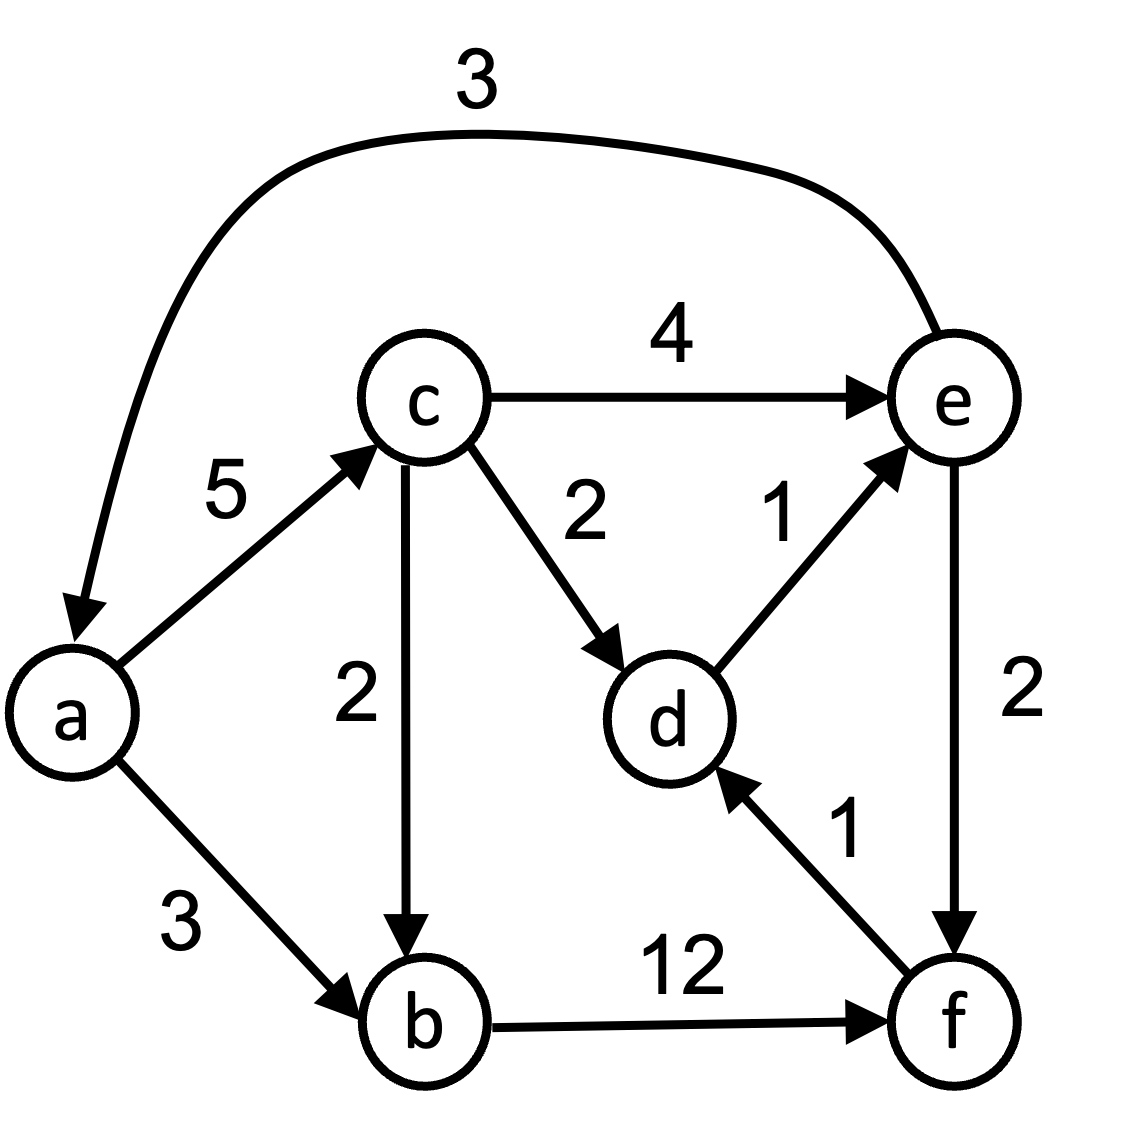
\includegraphics[width = .5\linewidth]{dijkstrasalg}
		\end{figure}
	
	
			\begin{figure}
				\centering
				\caption{Sample graph 2}
				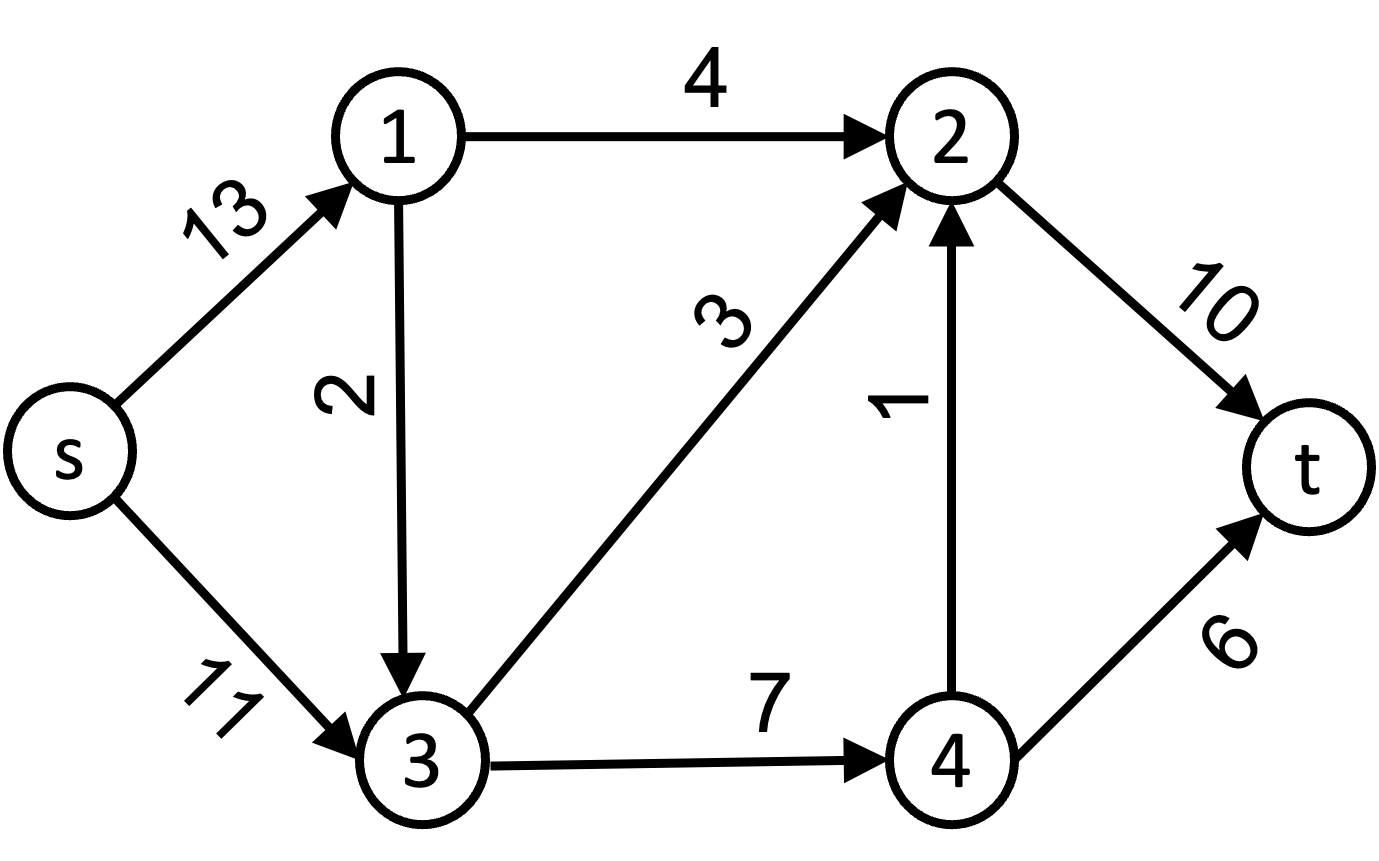
\includegraphics[width = .5\linewidth]{flow1}
			\end{figure}
		
					\begin{figure}
			\centering
			\caption{Sample graph 3}
			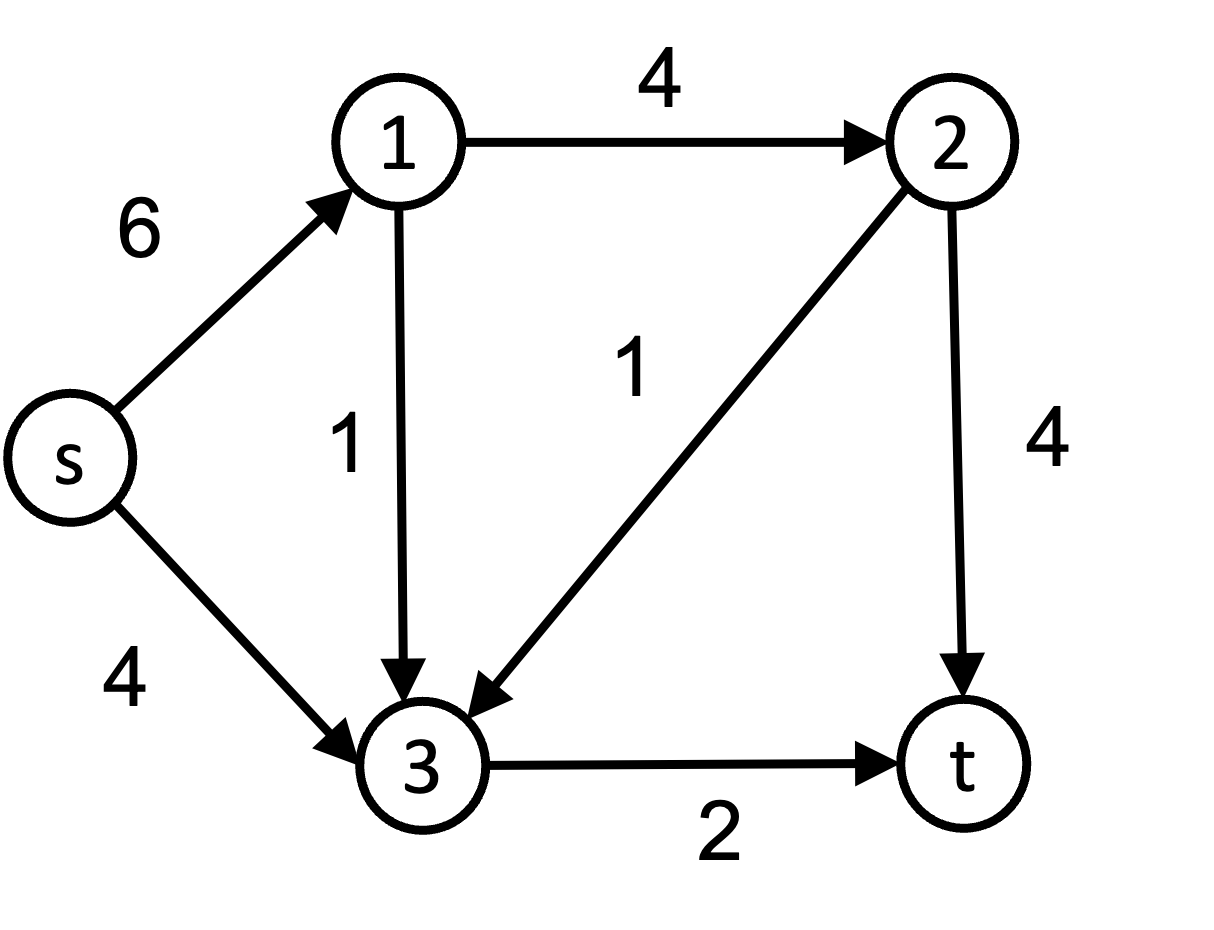
\includegraphics[width = .5\linewidth]{dag1}
		\end{figure}

	\end{questions}
\end{document}
